\documentclass[12pt,letterpaper]{article}

\usepackage[utf8]{inputenc}
\usepackage[T1]{fontenc}
\usepackage{amsmath}
\usepackage{amsfonts}
\usepackage{amssymb}
\usepackage{amsthm}
\usepackage[left=2cm,right=2cm,top=2cm,bottom=2cm,headheight=22pt]{geometry}
\usepackage{fancyhdr}
\usepackage{setspace}
\usepackage{lastpage}
\usepackage{graphicx}
\usepackage{caption}
\usepackage{subcaption}


\theoremstyle{definition}
\newtheorem{question}{Question}
\newtheorem{example}{Example}
\newtheorem{exercise}[question]{Exercise}
\newtheorem*{challenge}{Challenge}

\begin{document}

%Paramètres de mise en forme des paragraphes selon les normes françaises
\setlength{\parskip}{1ex plus 0.5ex minus 0.2ex}
\setlength{\parindent}{0pt}

%Paramètres relatifs aux en-têtes et pieds de page.
\pagestyle{fancy}
\lhead{Theron J Hitchman}
\chead{\Large Images for Meeting 06}
\rhead{Spring 2015}
\lfoot{\emph{Math and Decision Making}}
\cfoot{}
\rfoot{\emph{\thepage\ of \pageref{LastPage}}}


\section*{Pictures for Question 1: Which of these is a knot?}

\begin{figure}[h!]
    \begin{subfigure}[b]{0.4\textwidth}
        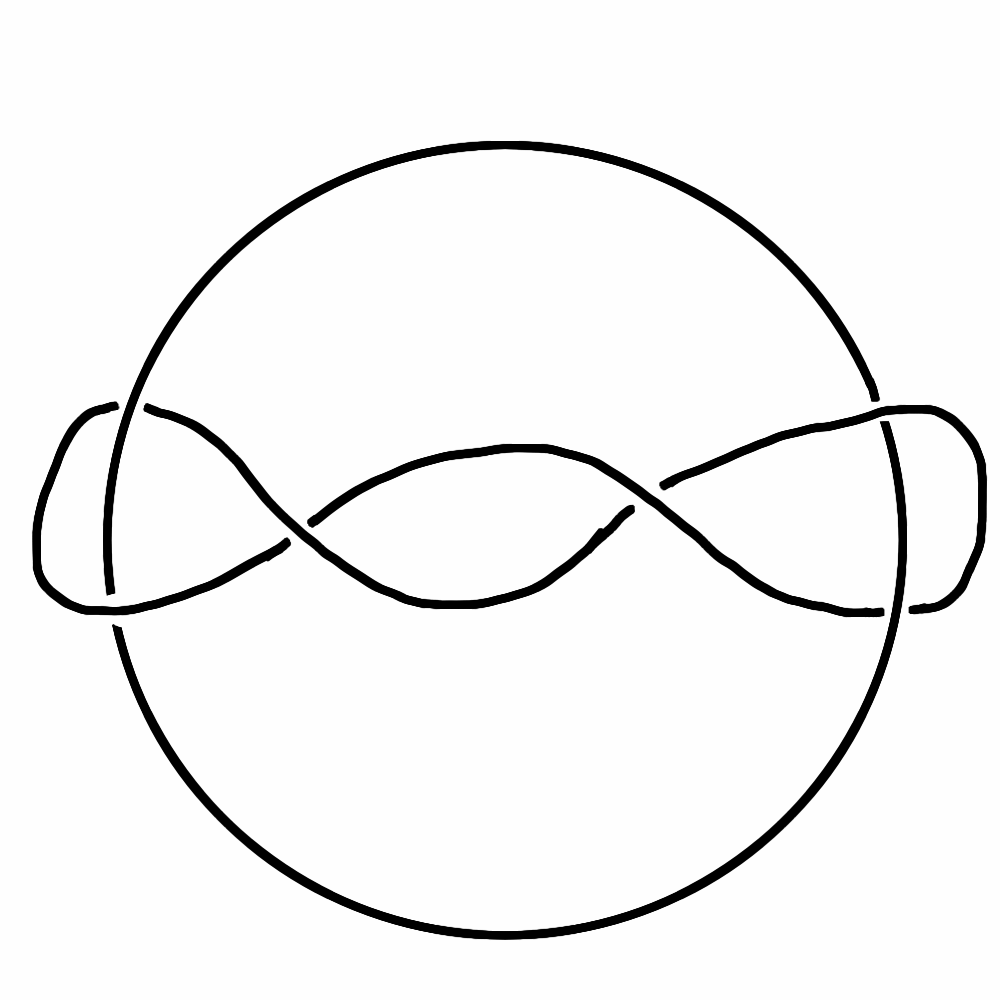
\includegraphics[width=\textwidth]{knotpics/9septQ1a.png}
        \caption{Choice A}
    \end{subfigure}
    \hspace{2cm}
    \begin{subfigure}[b]{0.4\textwidth}
        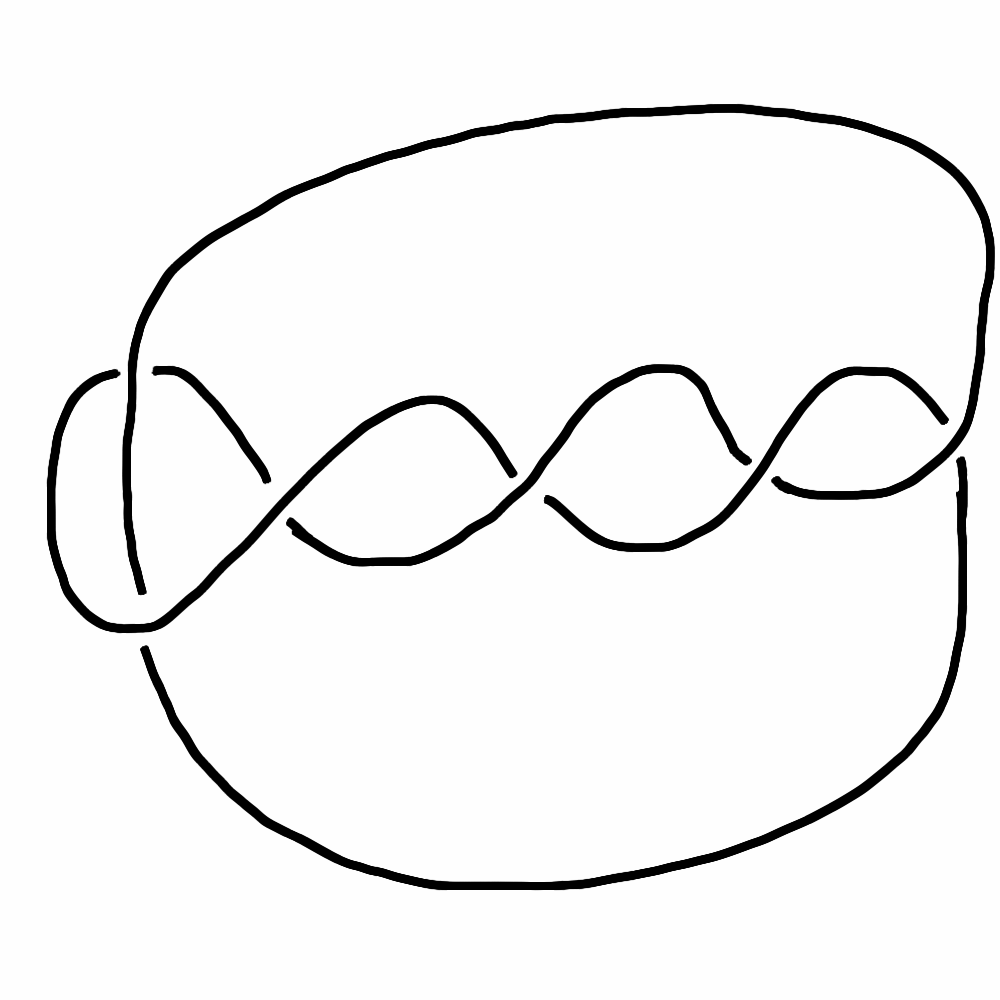
\includegraphics[width=\textwidth]{knotpics/9SeptQ1b.png}
        \caption{Choice B}
    \end{subfigure}
\end{figure}

\section*{Pictures for Question 2: Are these ``the same'' knot?}

\begin{figure}[h!]
    \begin{subfigure}[b]{0.4\textwidth}
        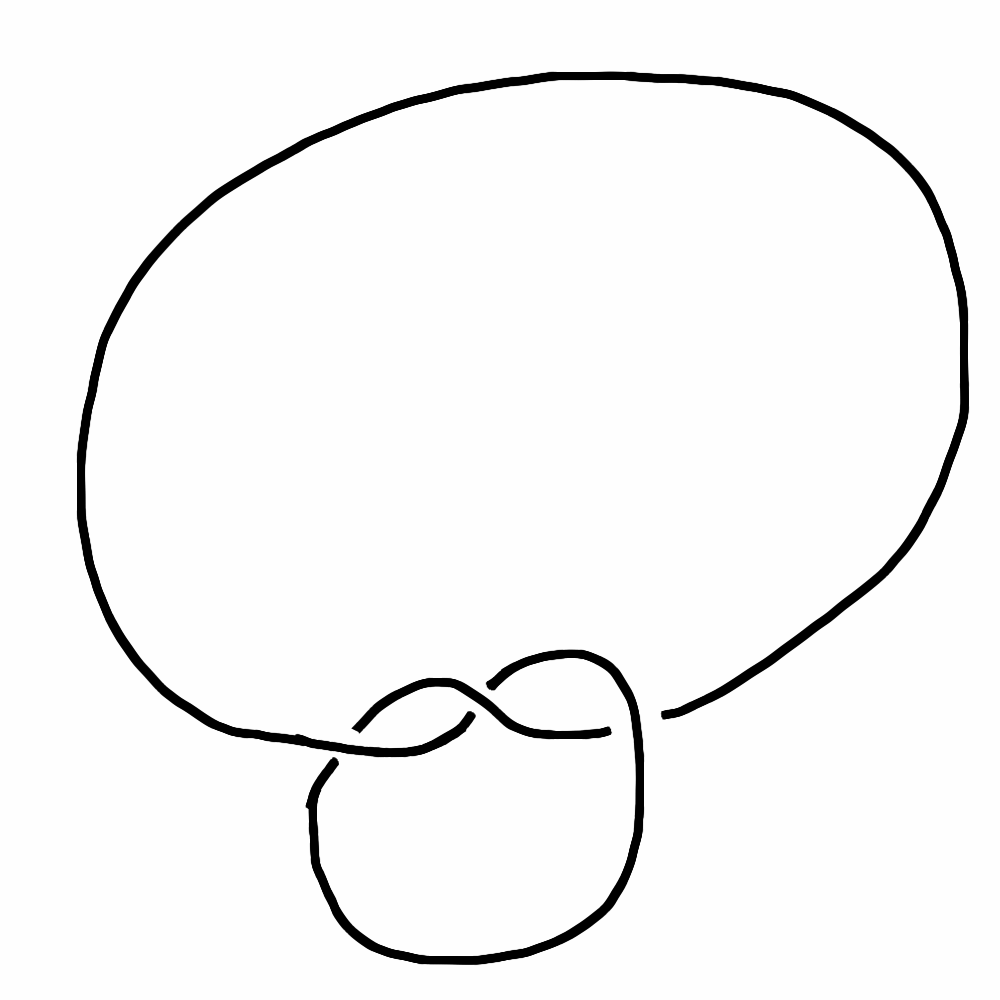
\includegraphics[width=\textwidth]{knotpics/9SeptQ2a.png}
        \caption{Choice A}
    \end{subfigure}
    \hspace{2cm}
    \begin{subfigure}[b]{0.4\textwidth}
        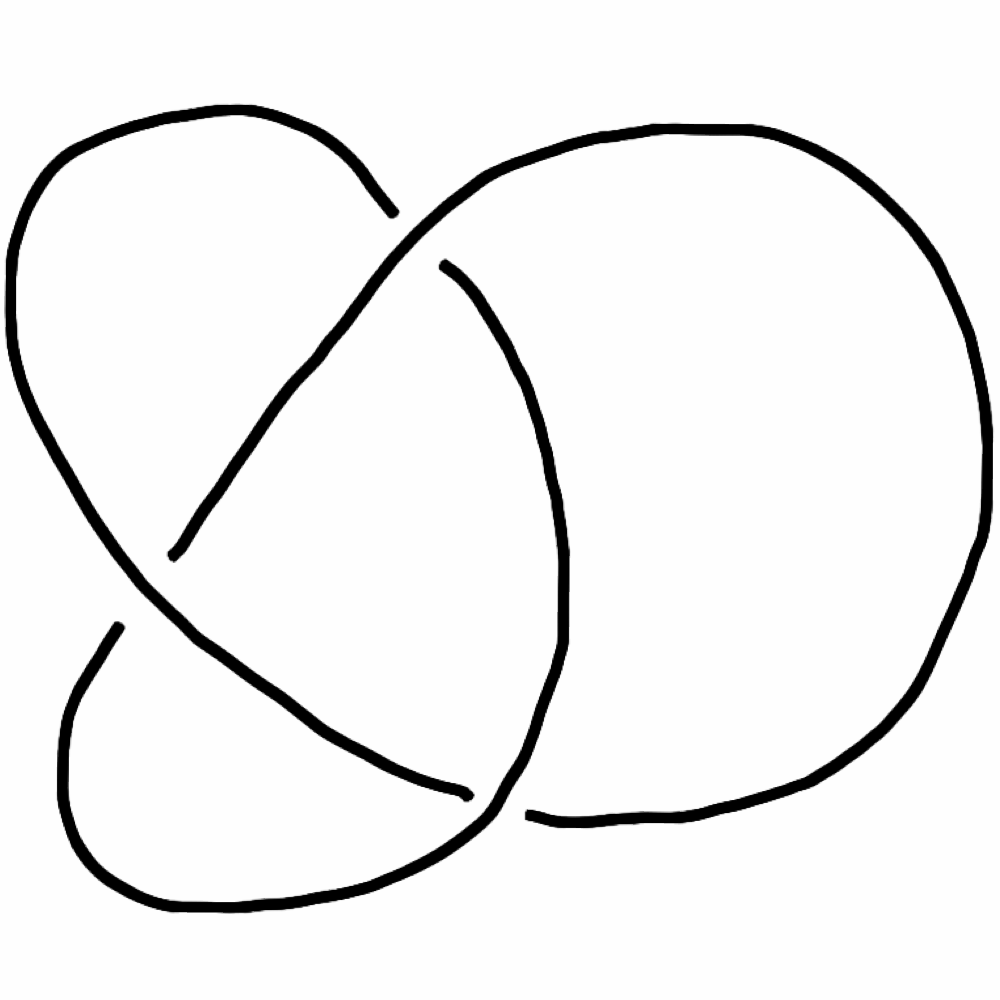
\includegraphics[width=\textwidth]{knotpics/9SeptQ2b.png}
        \caption{Choice B}
    \end{subfigure}
\end{figure}

\clearpage

\section*{Pictures for Question 3: Are these ``the same'' knot?}

\begin{figure}[h!]
    \begin{subfigure}[b]{0.4\textwidth}
        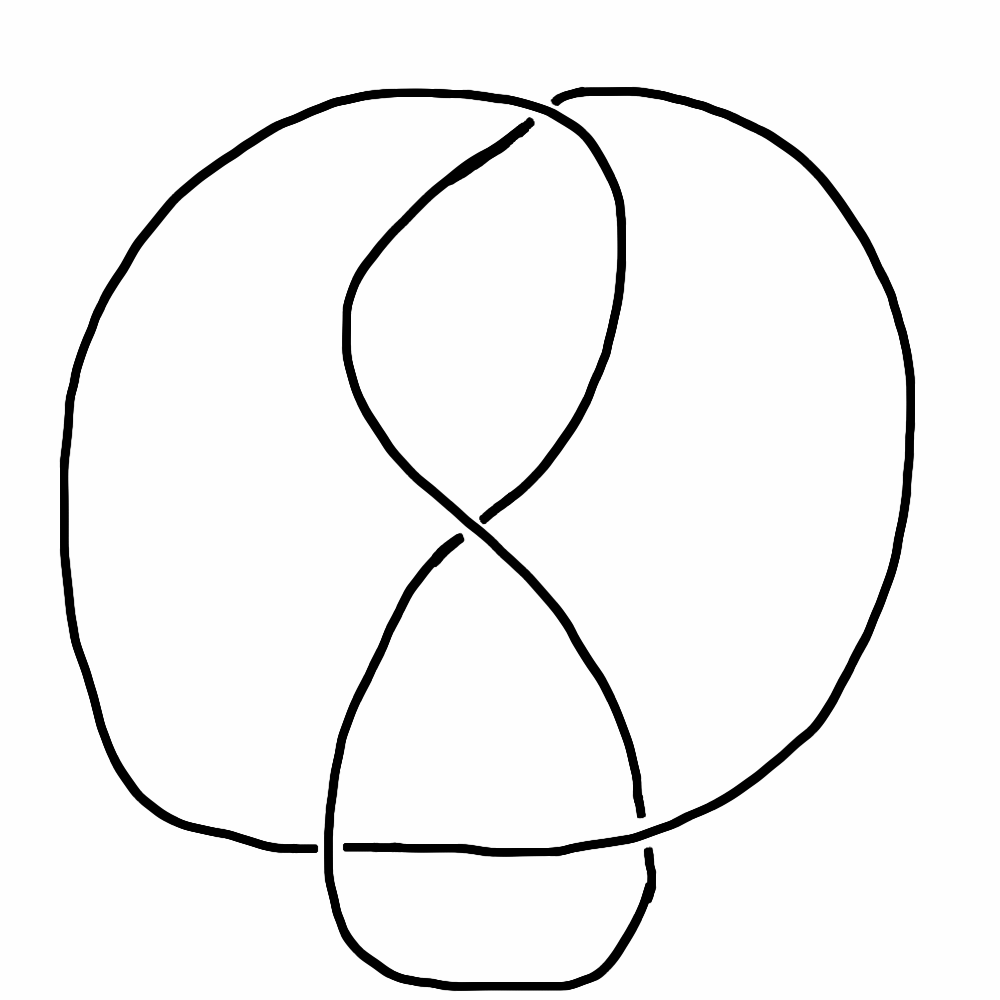
\includegraphics[width=\textwidth]{knotpics/9SeptQ3a.png}
        \caption{Choice A}
    \end{subfigure}
    \hspace{2cm}
    \begin{subfigure}[b]{0.4\textwidth}
        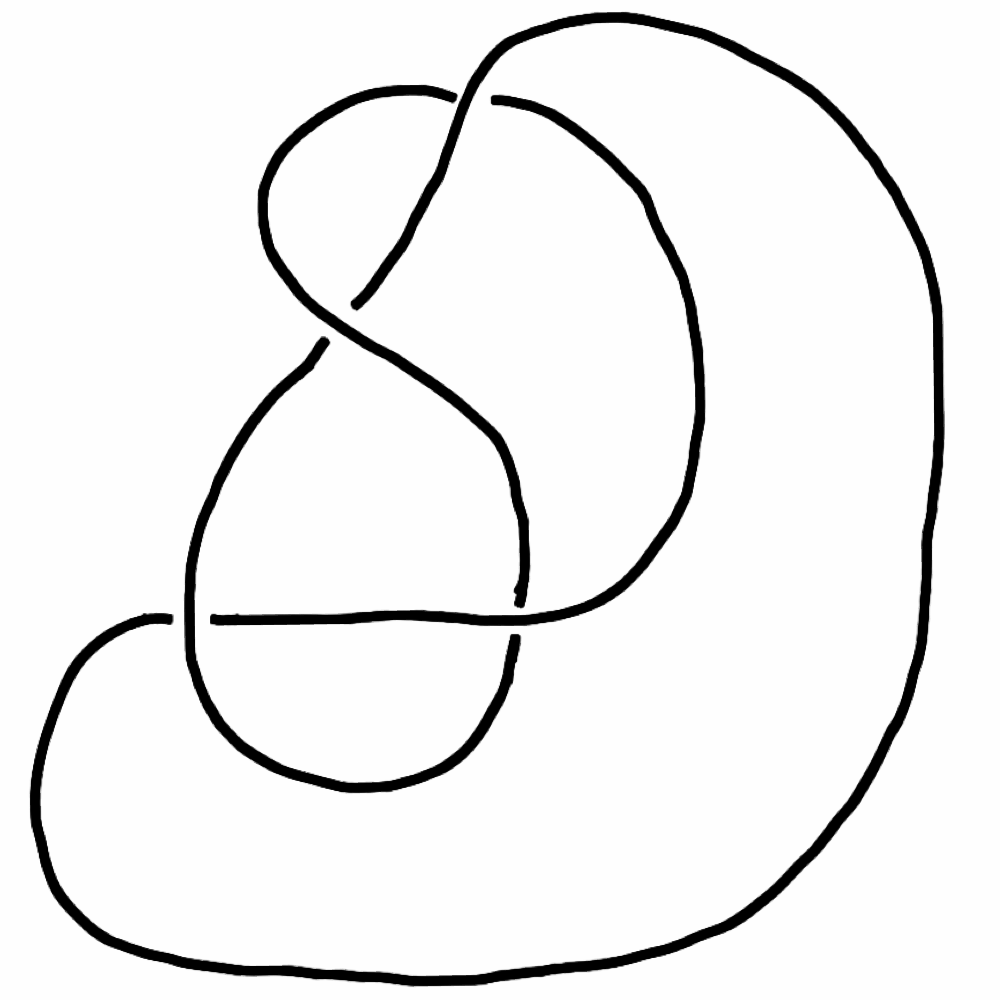
\includegraphics[width=\textwidth]{knotpics/9SeptQ3b.png}
        \caption{Choice B}
    \end{subfigure}
\end{figure}

\section*{Pictures for Question 4: Are these the ``the same'' knot?}

\begin{figure}[h!]
    \begin{subfigure}[b]{0.4\textwidth}
        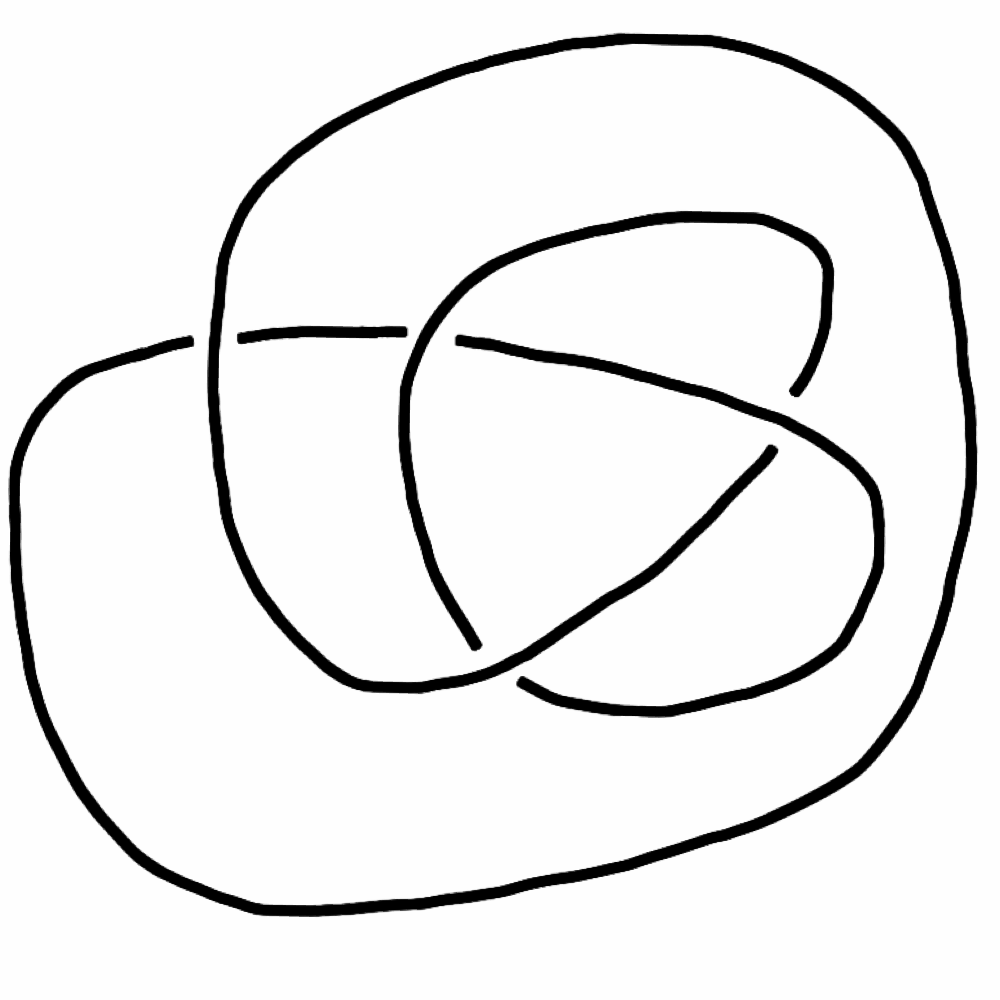
\includegraphics[width=\textwidth]{knotpics/9SeptQ4a.png}
        \caption{Choice A}
    \end{subfigure}
    \hspace{2cm}
    \begin{subfigure}[b]{0.4\textwidth}
        
\includegraphics[width=\textwidth]{knotpics/9SeptQ4b.png}
        \caption{Choice B}
    \end{subfigure}
\end{figure}

\clearpage

\section*{Pictures for Question 5: Are these ``the same'' knot?}

\begin{figure}[h!]
    \begin{subfigure}[b]{0.4\textwidth}
        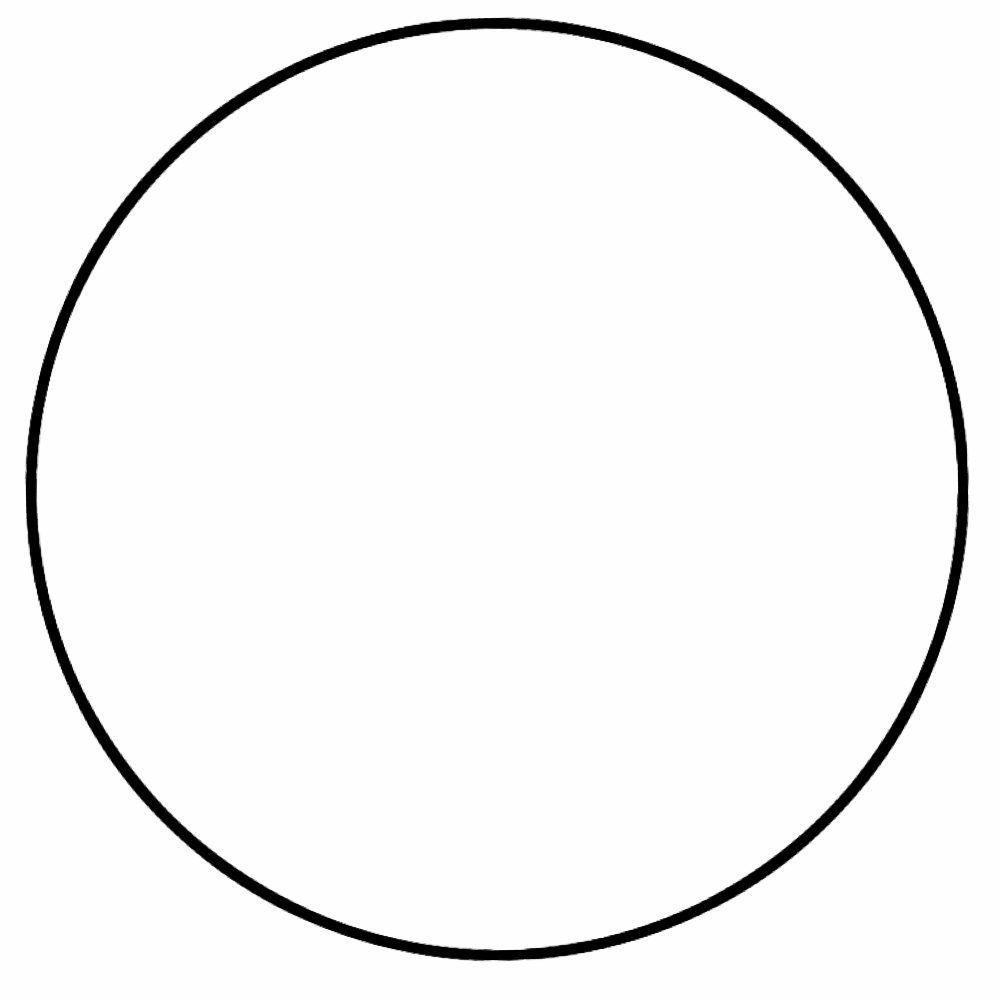
\includegraphics[width=\textwidth]{knotpics/9SeptQ5a.png}
        \caption{Choice A}
    \end{subfigure}
    \hspace{2cm}
    \begin{subfigure}[b]{0.4\textwidth}
        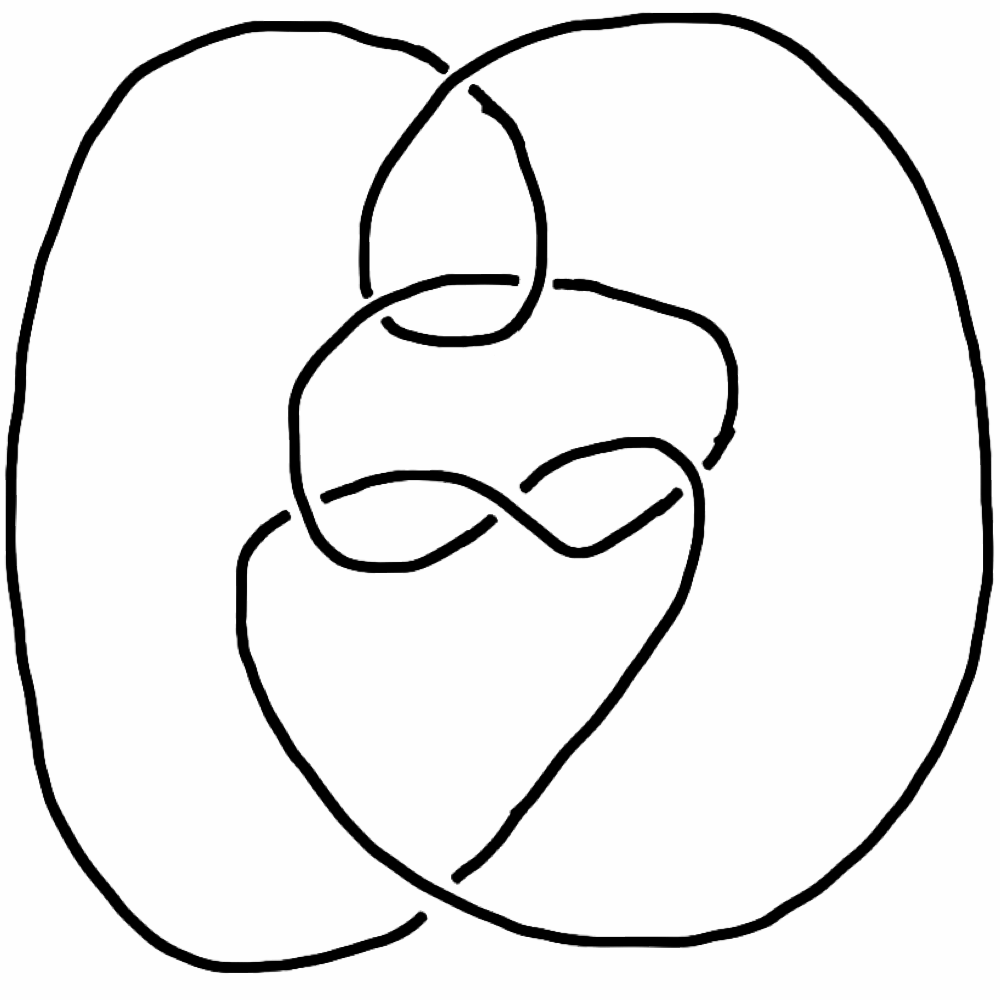
\includegraphics[width=\textwidth]{knotpics/9SeptQ5b.png}
        \caption{Choice B}
    \end{subfigure}
\end{figure}



\end{document}